\documentclass[a4paper, 12pt]{amsart}

\usepackage[utf8]{inputenc}
\usepackage{listings}
\usepackage{datetime}
\usepackage[margin=1.25in]{geometry}
\usepackage{tikz}
\usetikzlibrary{arrows}

\newdateformat{monthyeardate}{
  \monthname[\THEMONTH], \THEYEAR}

\title{A take on Neural Networks}
\author{Calad J.}
\author{Fonseca D.}
\author{Ortega A.}
\author{Marin M.}
\date{\today}

\begin{document}
\maketitle
\tableofcontents
\section{Basics on Neural Networks}
A neural network can be viewed as a directed graph in which each vertex serves
as a ``neuron'' that has an associated output value telling how active it is.
There will be two types of neurons of prime importance, these are inputs and
output neurons. The former simply takes the value of the input we will feed the
network with and the latter will be where we will collect the desired answer
from.\\
The simplest type of neural network there is and the one to be explored
in this document is called  a ``feedforward'' neural network. In this type of
networks all neurons are arranged by layers, where the only connections allowed
are between neurons in adjacent layers and information always travels from one
layer to the layer that comes next to it, never backwards (hence the
``feedforward'' term). This can be best seen in Figure
\ref{fig:feedforward example}.

\begin{figure}[!ht]
  \centering
  \def\layersep{2.5cm}

  \begin{tikzpicture}[shorten >=1pt,->,draw=black!50, node distance=\layersep]
    \tikzstyle{every pin edge}=[<-,shorten <=1pt]
    \tikzstyle{neuron}=[circle,draw,minimum size=17pt,inner sep=0pt]
    \tikzstyle{annot} = [text width=4em, text centered]

    % Draw the input layer nodes
    \foreach \y in {1,...,4}
    \node[neuron, pin=left:$x_\y$] (I-\y) at (0,-\y) {};

    % Draw the hidden layer nodes
    \foreach \y in {1,...,5}
    \path[yshift=0.5cm]
    node[neuron] (H-\y) at (\layersep,-\y cm) {};

    % Draw the output layer node
    \node[neuron,pin={[pin edge={->}]right:Output}, right of=H-3] (O) {};

    % Connect every node in the input layer with every node in the
    % hidden layer.
    \foreach \source in {1,...,4}
    \foreach \dest in {1,...,5}
    \path (I-\source) edge (H-\dest);

    % Connect every node in the hidden layer with the output layer
    \foreach \source in {1,...,5}
    \path (H-\source) edge (O);

    % Annotate the layers
    \node[annot,above of=H-1, node distance=1cm] (hl) {Hidden layer};
    \node[annot,left of=hl] {Input layer};
    \node[annot,right of=hl] {Output layer};
  \end{tikzpicture}
  \caption{Example of a feedforward neural network}
  \label{fig:feedforward example}
\end{figure}

In this type of neural networks the first layer will serve as input layer.
Similarly the last layer of such a network will serve as an output layer.
Intermediate layers are simply called ``hidden layers'' and will be treated
mostly as black boxes given that the activation values for these might not have
a clear interpretation even if the network produces highly accurate answers.

\begin{figure}[!ht]
  \centering
  \def\layersep{2.5cm}

  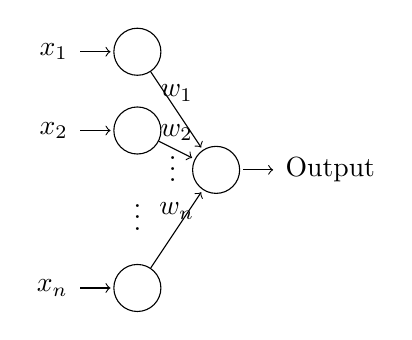
\begin{tikzpicture}[shorten >=1pt,->, node distance=\layersep]
    \tikzstyle{every pin edge}=[<-,shorten <=1pt]
    \tikzstyle{neuron}=[circle,draw,minimum size=17pt,
    inner sep=1pt]

    \node[neuron, pin=left:$x_1$] (I-1) at (0,-1) {};
    \node[neuron, pin=left:$x_2$] (I-2) at (0,-2) {};
    \node (D) at (0,-3) {$\vdots$};
    \node[neuron, pin=left:$x_n$] (I-n) at (0,-4) {};

    \node[neuron,pin={[pin edge={->}]right:Output}] (O) at (\layersep,-2.5){};

    \path (I-1) edge node [above] {$w_1$} (O)
          (I-2) edge node [above] {$w_2$} (O)
          (D)   edge [draw=none] node [above] {$\vdots$} (O)
          (I-n) edge node [above] {$w_n$} (O);

  \end{tikzpicture}
  \caption{Weights in a neural network}
  \label{fig:weights in a neural network}
\end{figure}

The activation value of a neuron in a given layer will be a function of the
activation values of neurons in the previous layer. It will also take into
account how important each of those neurons is to the neuron and a given bias of
it towards being activated or not. We can express this as follows:
\begin{equation*}
  a^l_i = f(b^l_i+\sum_{j=1}^{p}w^l_{i,j}a^{l-1}_j)
\end{equation*}
Where $a^l_i$ represents the activation value of neuron $i$ in layer $l$,
$b^l_i$ the associated bias with that neuron, $w^l_{i,j}$ the weight $a^l_i$
gives to $a^{l-1}_j$ and $f$ any arbitrary function. If we define $f$ of a
matrix as evaluating $f$ in each element of the matrix we can then expand this
into:

\begin{equation*}
  \begin{bmatrix}
    a^l_1\\
    a^l_2\\
    \vdots\\
    a^l_q
  \end{bmatrix}
  =
  f\left(
    \begin{bmatrix}
      w^l_{1,1} & w^l_{1,2} & \dots & w^l_{1,p}\\
      w^l_{2,1} & w^l_{2,2} & \dots & w^l_{2,p}\\
      \vdots    & \vdots    & \ddots& \vdots   \\
      w^l_{q,1} & w^l_{q,2} & \dots & w^l_{q,p}\\
    \end{bmatrix}
    \begin{bmatrix}
      a^{l-1}_1\\
      a^{l-1}_2\\
      \vdots\\
      a^{l-1}_p
    \end{bmatrix}
    +
    \begin{bmatrix}
      b^l_1\\
      b^l_2\\
      \vdots\\
      b^l_q
    \end{bmatrix}
  \right)\\
\end{equation*}
With $p$ and $q$ being the number of neurons in layers $l-1$ and $l$
respectively. Finally this can be written as:

\begin{equation*}
  \underset{q\times 1}{a^l}
  = f(\underset{q\times p}{W^l} \underset{p\times 1}{a^{l-1}}
  + \underset{q\times 1}{b^l})
\end{equation*}

For the sake of simplicity we will take:
\begin{align*}
  z^l &= W^la^{l-1}+b^l\\
  a^l &= f(z^l)
\end{align*}

The election of the activation function $f$ will highly influence the process
of training the neural network, making the process of finding a fitting $f$
important.
It is desired for this function to be monotonic increasing and differentiable
which will mean that increasing $z^l$ by a small value will also increase
$a^l$ by another small value.
Also, as any given layer can have an arbitrary number of neurons, $z^l$ could
take any real value. However it is desirable that $a^l$ is in some fixed range
in order to more easily handle the outputs of each neuron, and specially the
ones in the output layer.
It is common in the literature to chose as activation function a sigmoid curve,
and more specifically the logistic curve given by
\begin{equation*}
  \sigma(x)=\frac{1}{1+e^{-x}}
\end{equation*}
This we will use as our activation function, which makes our final network to
be characterized by
\begin{equation*}
  a^l=\sigma(z^l)
\end{equation*}

\section{Training the Network}
To train the network a initial test data set, composed by the input and the
expected output, is used. The objective is to compare the expected output and
the network's output, using the error function as proposed:

\begin{equation*}
  E(\hat{y}, y) = \frac{1}{2n}\sum_{i=1}^{n} (y_i-\hat{y_i})^2
\end{equation*}

With these results we can modify each weight and bias. This will result in the
network giving an output closer to the expected one. After many tests the
change in weights and biases will be determined by using the partial derivatives
of the cost function in respect to the weights and in respect to the biases,
resulting in the gradient which we seek to minimize in order to get the best
results:

\begin{equation*}
  \nabla C = \frac{\partial C}{\partial W}
\end{equation*}

To get the next position we desire to advance to we use these equations:

\begin{align*}
  w'_k &= w_k - \eta\frac{\partial C}{\partial w_k}\\
  b'_k &= b_k - \eta\frac{\partial C}{\partial b_k}
\end{align*}

Where $w_k$ are the network's weight, $b_k$ are the network's biases, and
$\eta$ is the learning factor which determines how far we will advance.

\begin{equation*}
  \begin{bmatrix}
    z_{1}^{l}\\
    z_{2}^{l}\\
    \vdots\\
    z_{n}^{l}
  \end{bmatrix}
   =
   \begin{bmatrix}
    w_{11} & w_{12} & w_{13} & \dots  & w_{1p} \\
    w_{21} & w_{22} & w_{23} & \dots  & w_{2p} \\
    \vdots & \vdots & \vdots & \ddots & \vdots \\
    w_{n1} & w_{n2} & w_{n3} & \dots  & w_{np}
\end{bmatrix}
   \begin{bmatrix}
    a_{1}^{l-1}\\
    a_{2}^{l-1}\\
    \vdots\\
    a_{p}^{l-1}
  \end{bmatrix}
  +
  \begin{bmatrix}
    b_{1}^{l}\\
    b_{2}^{l}\\
    \vdots\\
    b_{n}^{l}
  \end{bmatrix}
\end{equation*}

\begin{equation*}
  \begin{bmatrix}
    a_{1}^{l}\\
    a_{2}^{l}\\
    \vdots\\
    a_{n}^{l}
  \end{bmatrix}
   =
  \begin{bmatrix}
    \sigma(z_{1}^{l})\\
    \sigma(z_{2}^{l})\\
    \vdots\\
    \sigma(z_{n}^{l})
  \end{bmatrix}
\end{equation*}

\begin{figure}[!ht]
  \centering
  \def\layersep{2.5cm}

  \begin{tikzpicture}[shorten >=1pt,->,draw=black!50, node distance=\layersep]
    \tikzstyle{every pin edge}=[<-,shorten <=1pt]
    \tikzstyle{neuron}=[circle,draw,minimum size=17pt,inner sep=0pt]
    \tikzstyle{annot} = [text width=4em, text centered]

    % Draw the input layer nodes
    \foreach \y in {1,...,4}
    % This is the same as writing \foreach \name / \y in {1/1,2/2,3/3,4/4}
    \node[neuron, pin=left:$x_\y$] (I-\y) at (0,-\y) {};

    % Draw the hidden layer nodes
    \foreach \y in {1,...,5}
    \path[yshift=0.5cm]
    node[neuron] (H-\y) at (\layersep,-\y cm) {};

    % Draw the output layer node
    \foreach \y in {1,...,3}
    \path[yshift=-0.5cm]
    node[neuron, pin={[pin edge={draw=red,->}]right:$\hat{y}_\y$}] (J-\y) at (5cm,-\y cm) {};

    % Connect every node in the input layer with every node in the
    % hidden layer.
    \foreach \source in {1,...,4}
    \foreach \dest in {1,...,5}
    \path (I-\source) edge [draw=yellow] (H-\dest);

    % Connect every node in the hidden layer with the output layer
    \foreach \source in {1,...,5}
    \foreach \dest in {1,...,3}
    \path (H-\source) edge [draw=orange] (J-\dest);

    % Annotate the layers
    \node[annot,above of=H-1, node distance=1cm] (hl) {Hidden layer};
    \node[annot,left of=hl] {Input layer};
    \node[annot,right of=hl] {Output layer};
  \end{tikzpicture}
  \caption{Example of a neural network}
\end{figure}

\section{The Backpropagation Algorithm}

This algorithm computes the gradient of the cost function and updates weights
and biases as needed. Backpropagation is the core element of a neural network's
learning process. The relation with the partial derivatives of the cost function
comes from the base concept of backpropagation which is understanding how
changing weights and biases change the cost function. To understand it we first
need to assume the cost function can be written as an average of the cost
function for every test case. As described in the previous section, the error
function and cost function are the same. With this in mind, the assumption
states that the cost in the whole network is equivalent to the average of the
costs for each test:

\begin{equation*}
  C = \frac{1}{n}\sum_{i=1}^{n}C_i
\end{equation*}

Another important assumption is that the cost function can be written as a
function of the network's outputs:

\begin{equation*}
  C = C(a^l)
\end{equation*}

Our cost function satisfies this property as it can be written this way:

\begin{equation*}
  C = \frac{1}{2n}\sum_{i=1}^{n} (y_i-a_i^l)^2
\end{equation*}


The backpropagation algorithm also uses a not so common matrix operation,
called the Hadamard Product. This operation is denoted by the symbol $\bigodot$
and it refers to the element-wise product of a matrix.

An important value to define is called the error, represented by $\delta_j^l$,
where l is the layer and j is the neuron that contains this value. $\delta_j^l$
is a meaningful value because just by changing one neuron's error the total cost
will be modified. This value is defined as:

\begin{equation*}
  \delta_j^l = \frac{\partial C}{\partial z_j^l},\quad
  z^l_j = w_{jk}^la_k^{l-1}+b_j^l
\end{equation*}

Where l is the layer, j is the neuron in the $l^{th}$ layer and k is the neuron
in the $l-1^{th}$ layer.
\end{document}
